% This is "sig-alternate.tex" V2.1 April 2013
% This file should be compiled with V2.5 of "sig-alternate.cls" May 2012
%
% This example file demonstrates the use of the 'sig-alternate.cls'
% V2.5 LaTeX2e document class file. It is for those submitting
% articles to ACM Conference Proceedings WHO DO NOT WISH TO
% STRICTLY ADHERE TO THE SIGS (PUBS-BOARD-ENDORSED) STYLE.
% The 'sig-alternate.cls' file will produce a similar-looking,
% albeit, 'tighter' paper resulting in, invariably, fewer pages.
%
% ----------------------------------------------------------------------------------------------------------------
% This .tex file (and associated .cls V2.5) produces:
%       1) The Permission Statement
%       2) The Conference (location) Info information
%       3) The Copyright Line with ACM data
%       4) NO page numbers
%
% as against the acm_proc_article-sp.cls file which
% DOES NOT produce 1) thru' 3) above.
%
% Using 'sig-alternate.cls' you have control, however, from within
% the source .tex file, over both the CopyrightYear
% (defaulted to 200X) and the ACM Copyright Data
% (defaulted to X-XXXXX-XX-X/XX/XX).
% e.g.
% \CopyrightYear{2007} will cause 2007 to appear in the copyright line.
% \crdata{0-12345-67-8/90/12} will cause 0-12345-67-8/90/12 to appear in the copyright line.
%
% ---------------------------------------------------------------------------------------------------------------
% This .tex source is an example which *does* use
% the .bib file (from which the .bbl file % is produced).
% REMEMBER HOWEVER: After having produced the .bbl file,
% and prior to final submission, you *NEED* to 'insert'
% your .bbl file into your source .tex file so as to provide
% ONE 'self-contained' source file.
%
% ================= IF YOU HAVE QUESTIONS =======================
% Questions regarding the SIGS styles, SIGS policies and
% procedures, Conferences etc. should be sent to
% Adrienne Griscti (griscti@acm.org)
%
% Technical questions _only_ to
% Gerald Murray (murray@hq.acm.org)
% ===============================================================
%
% For tracking purposes - this is V2.0 - May 2012

\documentclass{sig-alternate-05-2015}

\usepackage{hyperref}

\begin{document}

% Copyright
%\setcopyright{acmcopyright}
%\setcopyright{acmlicensed}
%\setcopyright{rightsretained}
%\setcopyright{usgov}
%\setcopyright{usgovmixed}
%\setcopyright{cagov}
%\setcopyright{cagovmixed}


% DOI
%\doi{10.475/123_4}

% ISBN
%\isbn{123-4567-24-567/08/06}

%Conference
%\conferenceinfo{PLDI '13}{June 16--19, 2013, Seattle, WA, USA}

%\acmPrice{\$15.00}


%
% --- Author Metadata here ---
%\conferenceinfo{WOODSTOCK}{'97 El Paso, Texas USA}
%\CopyrightYear{2007} % Allows default copyright year (20XX) to be over-ridden - IF NEED BE.
%\crdata{0-12345-67-8/90/01}  % Allows default copyright data (0-89791-88-6/97/05) to be over-ridden - IF NEED BE.
% --- End of Author Metadata ---

\title{Business Intelligence, 188.429 WS 2016}
\subtitle{Assignment 1}
%
% You need the command \numberofauthors to handle the 'placement
% and alignment' of the authors beneath the title.
%
% For aesthetic reasons, we recommend 'three authors at a time'
% i.e. three 'name/affiliation blocks' be placed beneath the title.
%
% NOTE: You are NOT restricted in how many 'rows' of
% "name/affiliations" may appear. We just ask that you restrict
% the number of 'columns' to three.
%
% Because of the available 'opening page real-estate'
% we ask you to refrain from putting more than six authors
% (two rows with three columns) beneath the article title.
% More than six makes the first-page appear very cluttered indeed.
%
% Use the \alignauthor commands to handle the names
% and affiliations for an 'aesthetic maximum' of six authors.
% Add names, affiliations, addresses for
% the seventh etc. author(s) as the argument for the
% \additionalauthors command.
% These 'additional authors' will be output/set for you
% without further effort on your part as the last section in
% the body of your article BEFORE References or any Appendices.

\numberofauthors{2} %  in this sample file, there are a *total*
% of EIGHT authors. SIX appear on the 'first-page' (for formatting
% reasons) and the remaining two appear in the \additionalauthors section.
%
\author{
% You can go ahead and credit any number of authors here,
% e.g. one 'row of three' or two rows (consisting of one row of three
% and a second row of one, two or three).
%
% The command \alignauthor (no curly braces needed) should
% precede each author name, affiliation/snail-mail address and
% e-mail address. Additionally, tag each line of
% affiliation/address with \affaddr, and tag the
% e-mail address with \email.
%
% 1st. author
\alignauthor
Stefan Beyer\\
       \affaddr{Student ID: 1225423}\\
       \email{e1225423@student.tuwien.ac.at}
% 2nd. author
\alignauthor
Georg Heiler\\
       \affaddr{Student ID: 1225063}\\
       \email{e1225063@student.tuwien.ac.at}
}
% There's nothing stopping you putting the seventh, eighth, etc.
% author on the opening page (as the 'third row') but we ask,
% for aesthetic reasons that you place these 'additional authors'
% in the \additional authors block, viz.
\date{30 July 1999}
% Just remember to make sure that the TOTAL number of authors
% is the number that will appear on the first page PLUS the
% number that will appear in the \additionalauthors section.

\maketitle

\section{Dataset}
We use the \href{https://www.kaggle.com/c/leaf-classification}{leaf classification dataset from Kaggle}. The idea is to automate plant recognition. The data consists of binary leaf images and extracted features, including shape, margin \& texture, to accurately identify 99 species of plants.

\subsection{Characteristics of the extracted features}
The following numbers are for the training data set

\begin{itemize}
  \item Number of features 194
  \item Number of categorical features 1
  \item Number of numerical features 193
  \item Number of Samples 990
  \item Target variable contains 99 different species
\end{itemize}

The test data set contains 594 additional instances. All in all the minimum requirements for the dataset are fulfilled.


A detailed description of mean / min values or value ranges can be found in 
\textbf{firstAnalysisOfTheData}
, including histograms. 

In general:
\begin{enumerate}
  \item id
  \item ID of the images from which the features were extracted
  \item Range: [1,1584]
  \item marginN (1-64)
  \begin{enumerate}
	  \item Numerical
	  \item Range (approximately): [0,0.3]
	  \item Many outliers
  \end{enumerate}
  \item shapeN (1-64)
  \begin{enumerate}
 	  \item Numerical
	  \item Range (approximately): [0,0.003]
	  \item Few outliers
\end{enumerate}
\item textureN (1-64)
	\begin{enumerate}
		\item Numerical
	  \item Range (approximately): [0,0.43]
	  \item Few outliers
\end{enumerate}

\item species
  \begin{enumerate}
	\item Categorical
	  \item 99 unique values
	  \item The dataset does not contain any missing values and is not sparse.
\end{enumerate}

\end{enumerate}

\section{Classification}
Analysis of Train/Test Set Splits, Performance and Parameters

\subsection{Selection of algorithms}
\subsubsection{Logistic regression (extracted features)}
\begin{enumerate}
  \item results easy to interpret
  \item fast to compute
\end{enumerate}

\subsubsection{Random forest (extracted features)}
\begin{enumerate}
  \item popular methodology
  \item no feature scaling required
  \item very robust
  \item quick for smaller datasets
\end{enumerate}

\subsection{Preprocessing}
\subsubsection{Scaling}
marginN, scaleN and textureN will be scaled. 
\subsubsection{OWN}
For marginN and textureN we will introduce a new column with binary values which will be 1 if the value of marginN/textureN is nearly 0.
We do this in order to better handle numeric distances which otherwise might get distorted.

\subsection{Subsampling}
We will process the entire dataset, as it only contains around 1000 rows.

\section{Foo}
\begin{figure}[]
  \centering
  \caption{Logistic regression with TODO settings}
  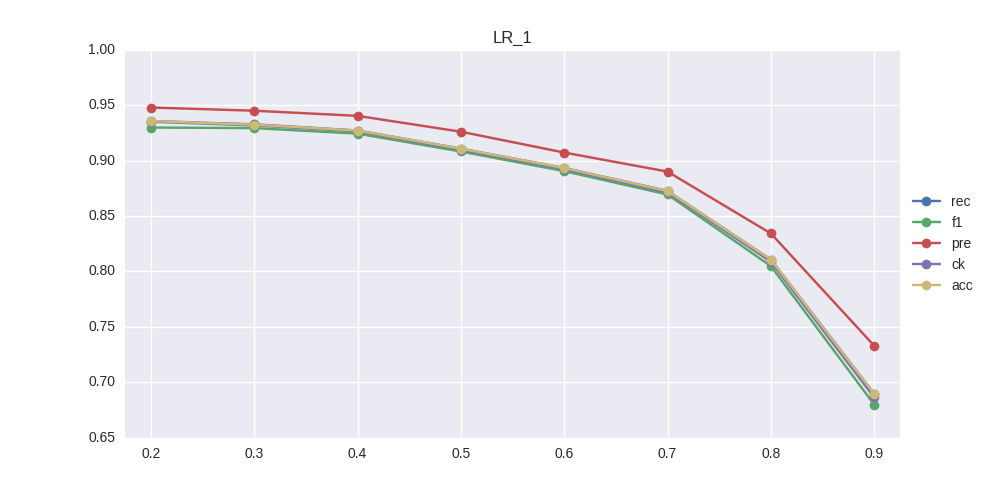
\includegraphics[width=\textwidth]{../plots/LR_1}
  \label{fig:anomalySetup}
\end{figure}

\end{document}
